\clearpage
\section{Paired transfer uncertainty and numerical cases}
\label{app:derived-transfer}
We analyze the saved query-level predictions in \path{data/transfer_queries.csv} (L46). Source key R01 maps the derived results to \path{revision/derived_transfer_analysis.json}; \path{scripts/prepare_revision.py} regenerates them.

\subsection{Exact paired sequence bootstrap}
The analysis uses the 468 eligible Extended-new predictions and their 32 physical-sequence groups. Each of 10,000 replicates samples 32 group identities with replacement and includes every query from each sampled group. Repeated groups contribute repeated queries. PHASE-TTC and RGB share the sampled indices. For each model, we compute pooled mean, median, and 95th-percentile absolute error, then form the PHASE-minus-RGB difference. NumPy's \texttt{linear} quantile convention and \texttt{default\_rng(20261028)} define the 2.5th and 97.5th percentile endpoints.

The point differences are \RevisionMeanDelta\,s for the mean, \RevisionMedianDelta\,s for the median, and \RevisionPninetyfiveDelta\,s for p95. All three intervals contain zero (Table~\ref{tab:revision-bootstrap}). The exploratory intervals condition on the fitted models and development-exposed sequences; they do not incorporate representation-training variability or adaptive model selection.

Differences use full-precision predictions. The mean difference rounds to $+0.007$\,s; subtracting the separately rounded means 1.023 and 1.015 instead gives $+0.008$\,s.

\subsection{Numerical cases}
The two queries below maximize and minimize the PHASE-minus-RGB absolute-error difference within the saved predictions. These post hoc examples show the range of model disagreement; their causes would require inspection of the corresponding sensor observations.
\begin{table}[H]\centering\small
\caption{Queries with the largest positive and negative PHASE-minus-RGB absolute-error differences in the labeled transfer set. \evidence{R01,L46}}
\label{tab:revision-cases}
\begin{tabularx}{\linewidth}{@{}Xrrrr@{}}\toprule
Query & Target (s) & PHASE (s) & RGB (s) & $\Delta$ AE (s)\\\midrule
{\footnotesize\path{CPNAO-high:13700430}} & 2.996 & 6.604 & -12.903 & -12.290\\
{\footnotesize\path{CCRs-1-medium-100-overlap-100:5950352}} & 6.765 & -25.740 & -9.880 & +15.861\\
\bottomrule\end{tabularx}\end{table}
\FloatBarrier

\clearpage
\subsection{Complete sequence comparisons}
\begin{figure}[H]
\centering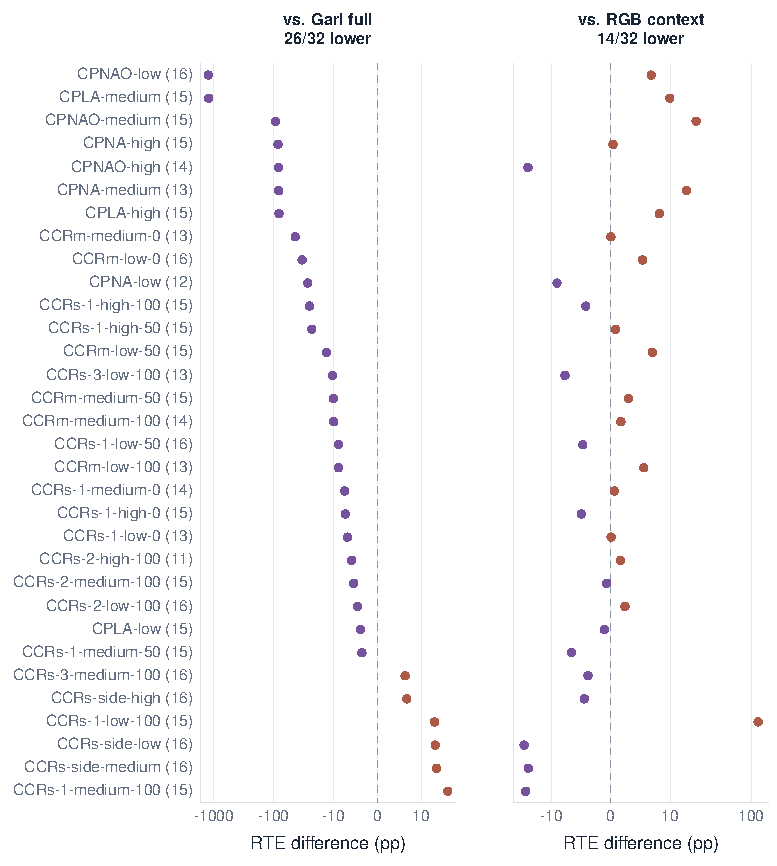
\includegraphics[width=\linewidth,height=.70\textheight,keepaspectratio]{figures/rev_sequence.pdf}
\caption{\textbf{Sequence-level relative TTC error differences.} Both panels show the 32 labeled Extended-new sequences in a common order; parentheses give query counts and negative values favor PHASE-TTC. The symmetric-log axes are linear between $-5$ and $+5$ percentage points. Display labels omit repeated overlap suffixes; Table~\ref{tab:sequence-full} gives the full identities. \evidence{R01,L46}}
\label{fig:transfer-sequence}
\end{figure}
\FloatBarrier
\clearpage
{\small\begin{longtable}{@{}p{6.0cm}rrrrr@{}}
\caption{Query counts and mean RTE (\%) for all 32 Extended-new sequences. Differences are in percentage points. \evidence{R01,L46}}\label{tab:sequence-full}\\
\toprule Sequence & $n$ & PHASE & RGB & Garl & $\Delta_{\rm RGB}$\\\midrule\endfirsthead
\toprule Sequence & $n$ & PHASE & RGB & Garl & $\Delta_{\rm RGB}$\\\midrule\endhead
\bottomrule\endfoot
CPNAO-low & 16 & 46.95 & 41.09 & 1283.26 & +5.86\\
CPLA-medium & 15 & 45.43 & 35.53 & 1265.98 & +9.90\\
CPNAO-medium & 15 & 41.92 & 20.94 & 134.36 & +20.98\\
CPNA-high & 15 & 66.50 & 66.14 & 150.71 & +0.36\\
CPNAO-high & 14 & 55.86 & 75.18 & 137.89 & -19.31\\
CPNA-medium & 13 & 59.61 & 43.68 & 141.20 & +15.93\\
CPLA-high & 15 & 62.29 & 54.92 & 143.22 & +7.37\\
CCRm-medium-0-overlap-0 & 13 & 14.61 & 14.57 & 57.78 & +0.04\\
CCRm-low-0-overlap-0 & 16 & 16.40 & 11.85 & 49.69 & +4.56\\
CPNA-low & 12 & 35.90 & 44.34 & 62.54 & -8.44\\
CCRs-1-high-100-overlap-100 & 15 & 19.23 & 22.75 & 44.19 & -3.52\\
CCRs-1-high-50-overlap-50 & 15 & 18.25 & 17.55 & 41.09 & +0.71\\
CCRm-low-50-overlap-50 & 15 & 17.70 & 11.67 & 30.65 & +6.02\\
CCRs-3-low-100-overlap-100 & 13 & 8.35 & 15.08 & 18.67 & -6.73\\
CCRm-medium-50-overlap-50 & 15 & 20.93 & 18.41 & 30.93 & +2.53\\
CCRm-medium-100-overlap-100 & 14 & 15.25 & 13.79 & 25.04 & +1.47\\
CCRs-1-low-50-overlap-50 & 16 & 4.98 & 8.93 & 13.15 & -3.95\\
CCRm-low-100-overlap-100 & 13 & 20.69 & 15.96 & 28.85 & +4.73\\
CCRs-1-medium-0-overlap-0 & 14 & 6.72 & 6.17 & 13.14 & +0.55\\
CCRs-1-high-0-overlap-0 & 15 & 17.32 & 21.49 & 23.61 & -4.17\\
CCRs-1-low-0-overlap-0 & 13 & 9.81 & 9.73 & 15.58 & +0.07\\
CCRs-2-high-100-overlap-100 & 11 & 13.75 & 12.35 & 18.65 & +1.40\\
CCRs-2-medium-100-overlap-100 & 15 & 6.84 & 7.39 & 11.36 & -0.55\\
CCRs-2-low-100-overlap-100 & 16 & 15.67 & 13.62 & 19.44 & +2.05\\
CPLA-low & 15 & 25.19 & 26.09 & 28.38 & -0.90\\
CCRs-1-medium-50-overlap-50 & 15 & 5.73 & 11.32 & 8.66 & -5.60\\
CCRs-3-medium-100-overlap-100 & 16 & 15.32 & 18.54 & 9.91 & -3.21\\
CCRs-side-high & 16 & 21.54 & 25.26 & 15.77 & -3.72\\
CCRs-1-low-100-overlap-100 & 15 & 395.63 & 273.53 & 378.78 & +122.10\\
CCRs-side-low & 16 & 41.76 & 63.28 & 24.48 & -21.52\\
CCRs-side-medium & 16 & 46.06 & 65.11 & 27.92 & -19.05\\
CCRs-1-medium-100-overlap-100 & 15 & 111.28 & 131.87 & 83.19 & -20.60\\
\end{longtable}}

